\subsection{Architecture générale}

Le transformeur a une architecture encodeur--décodeur (Voire Figure~\ref{fig.transformer}).
L'encodeur et le décodeur ont des architectures très similaires, 
comprenant chacun une couche d'encodage positionnel, une couche d'auto-attention et un \gls{mlp}.
Le décodeur se distingue de l'encodeur 
en ce qu'il a une couche d'attention croisée entre l'auto-attention et l'\gls{mlp}.
Chacune des couches susmentionnées est suivie d'une couche de normalisation~\cite{Ba_Kiros_Hinton_2016}
qui reçoit également une connexion directe à l'entrée de la couche%
\footnote{%
    On parle de connexion résiduelle ou de connexion de saut \foreignlanguage{english}{(skip connection)}.
}.
L'encodeur et le décodeur peuvent être empilés pour former un transformeur profond.

\begin{figure}[htb]
    \centering
    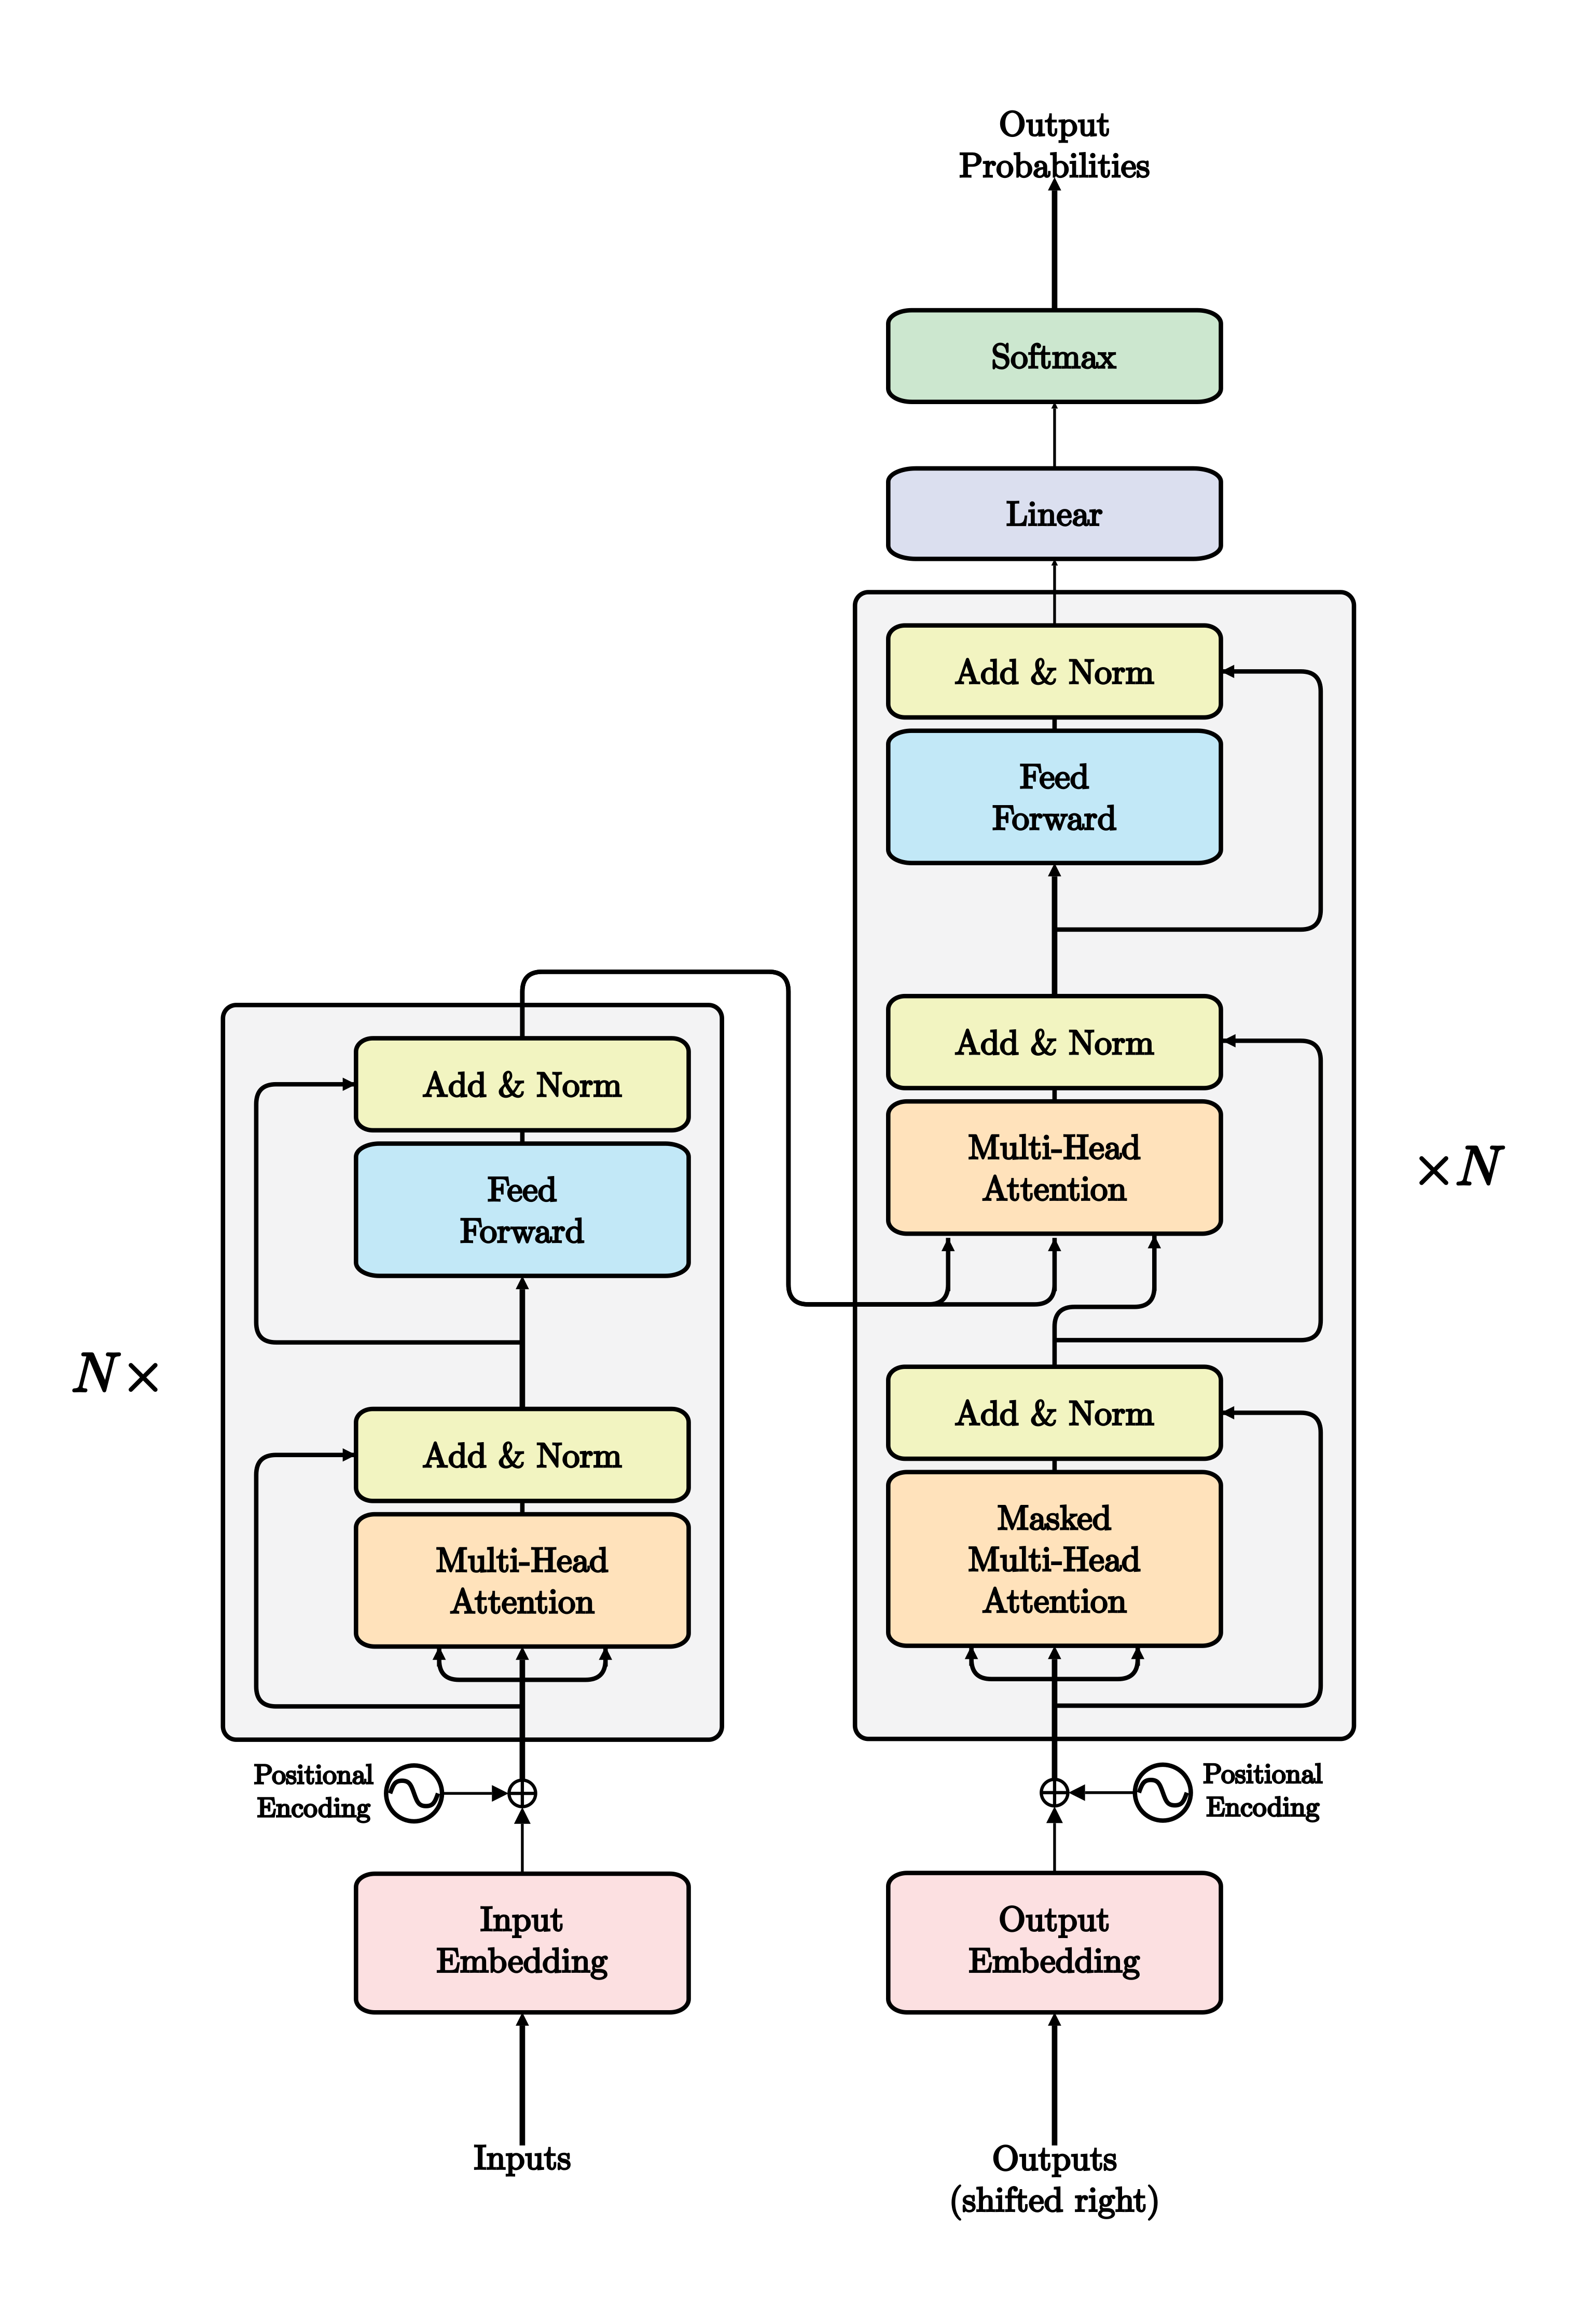
\includegraphics[width=8cm]{assets/images/transformer.png}
    \caption[L'architecture de transformeur.]
    {L'architecture de transformeur~\cite[Fig 1]{attention}.}
    \label{fig.transformer}
\end{figure}

Étant donné une séquence d'entrée \(x = (x_1, \ldots, x_n)\),
l'encodeur calcule un vecteur de pensée \(z\) qu'il passe au décodeur.
Le décodeur prédit le prochain élément \(y_i\) de la séquence de sortie 
à partir de \(z\) et les éléments précédents \((y_1, \ldots, y_{i-1})\).
Pour produire \(y_0\), le décodeur commence avec une séquence de sortie vide.
